\documentclass[UTF8]{ctexart}
\usepackage{ctex}
\usepackage{amsthm,amsmath,amssymb}
\usepackage{color}
\usepackage[colorlinks,linkcolor=red]{hyperref}
\usepackage{mathrsfs}
\usepackage{boondox-cal}
\usepackage{braket}
\usepackage{graphicx}
\usepackage{epstopdf}
\usepackage{dutchcal}
\usepackage{lmodern}
\newcommand{\rank}{\mathrm{rank}}

\title{Chap 4}
\author{}
\date{}
\pagestyle{plain}
\begin{document}
	\maketitle
    \section*{4 数据分析过程}
	上接分类...

    \subsection*{网络的构建}
	\subsubsection*{简单的情形: 对分类的检验, 使用神经网络的可行性}
	上面我们已经给出了聚类分析. 我们自然想要知道的是我们的分类是否正确地指导了我们对于疫情的解读? 出于此目的, 使用神经网络工具箱, 我们可以简单地搭建一个网络: 网络结构用 MATLAB 的格式简单地例举如下.
	\begin{align*}
		&\text{sequenceInputLayer(8)} \rightarrow \\
    	&\text{fullyConnectedLayer(300)} \rightarrow \\
    	&\text{reluLayer} \rightarrow \\
    	&\text{fullyConnectedLayer(300)} \rightarrow \\
    	&\text{reluLayer} \rightarrow \\
    	&\text{fullyConnectedLayer(300)} \rightarrow \\
    	&\text{reluLayer} \rightarrow \\
    	&\text{fullyConnectedLayer(numResponses)} \rightarrow \\
    	&\text{regressionLayer}
	\end{align*}
	这里这个网络用于预测每日新增的病例. 传入的单个数据将是
	\[
	\begin{bmatrix}
		\text{当前总感染人数}\\
		\text{前4日新增人数}\\
		\text{前3日新增人数}\\
		\text{前2日新增人数}\\
		\text{前1日新增人数}\\
		\text{PCA 截断值1}\\
		\text{PCA 截断值2}\\
		\text{PCA 截断值3}
	\end{bmatrix}
	\]
	用于对后一日的新增病例个数进行预测. 值得提到的是, 正如前面所说, 这里我们将新增病例个数进行了光滑化. 具体地, 记新增病例数所称的向量为 $\mathcal{N}$, 我们使用
	\[
		\mathcal{N}_{\mathcal{S}} = \text{conv}(\mathcal{N},\mathcal{K}), \quad \mathcal{K} = \begin{bmatrix}
			\displaystyle\frac{1}{4}&\displaystyle\frac{1}{4}&\displaystyle\frac{1}{4}&\displaystyle\frac{1}{4}
	\end{bmatrix}
	\]
	作为我们认为的新增病例数.

	这里我们的选取是之前提到分类中的第二类的部分国家, 也即 France, South Korea, Australia, Canada, Iceland. 我们选取 Adam 优化器, 对上述数据训练 4000 个 epoches. 选取的用于验证的国家为 Saudi Arabia, Germany, Japan, United States. 初始的学习率设置为 $0.001$, 并每 75 个 epoch 乘以 $0.95$.

	为了说明我们的网络是工作的, 我们给出其在训练集上的效果(当然, 这样的测试并不令人信服):
	\begin{figure}[htbp]
	    \centering
	    \subfigure{
	    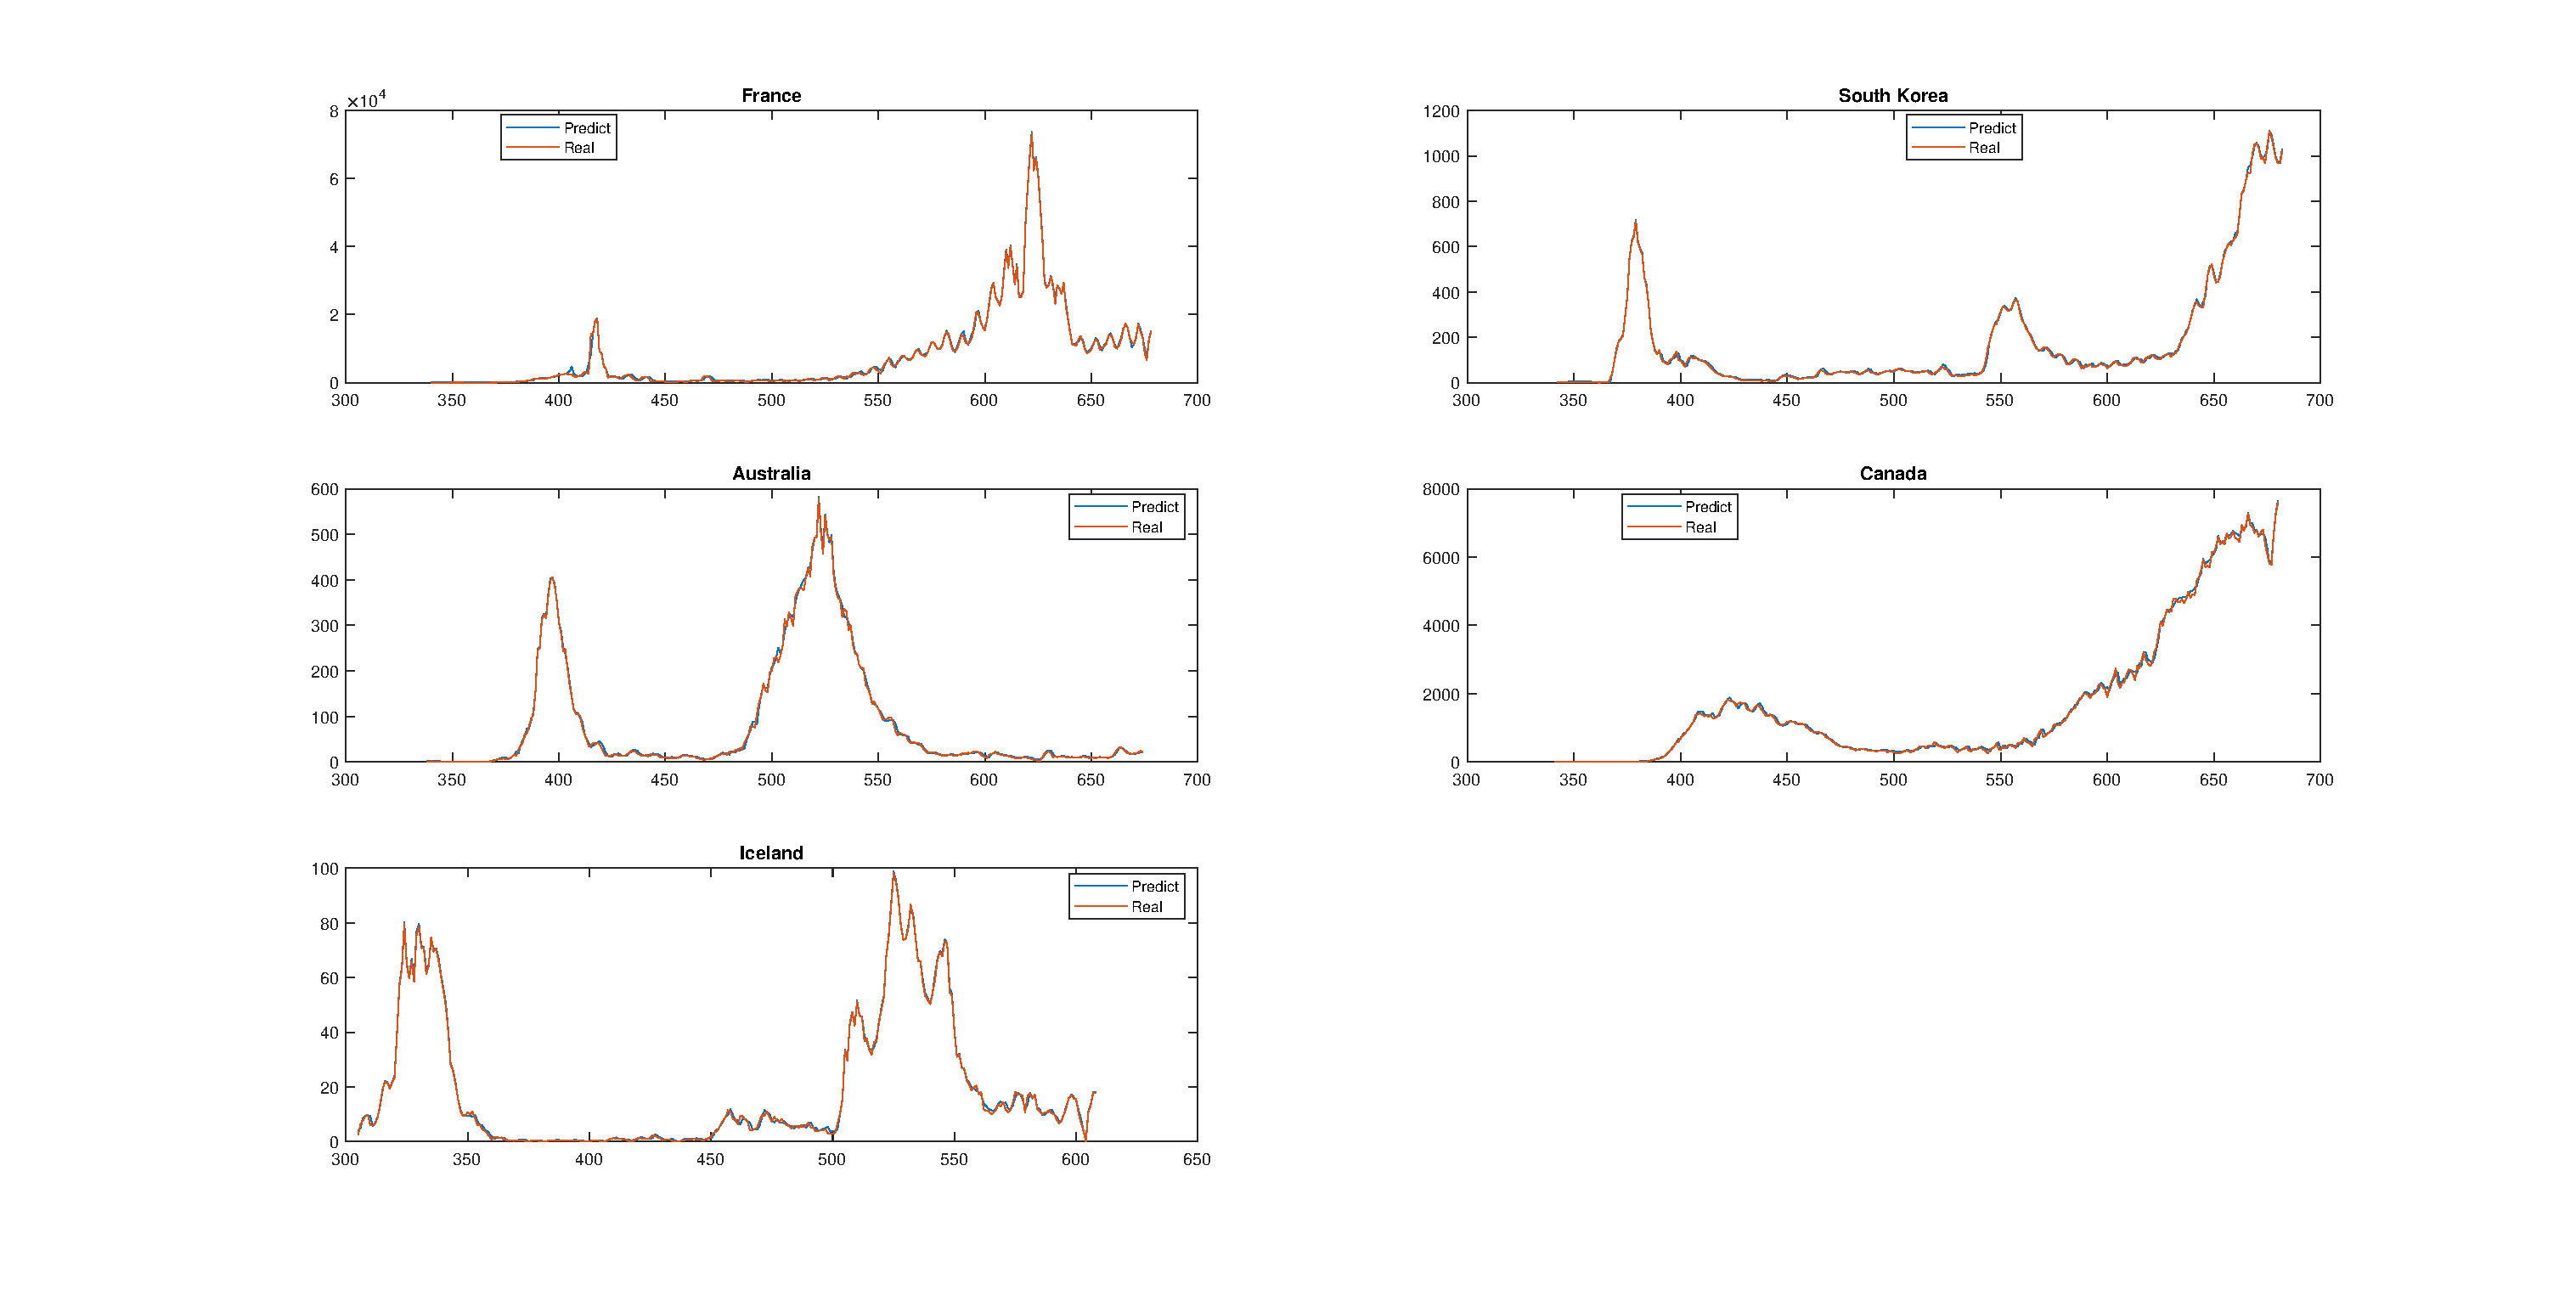
\includegraphics[height=12cm, width=14cm]{trainset.eps}
	    }
	\end{figure}

	对于测试集, 我们选取 Saudi Arabia, Germany, Japan, United States 四个国家. 所得到的预测结果见下图:
	\begin{figure}[htbp]
	    \centering
	    \subfigure{
	    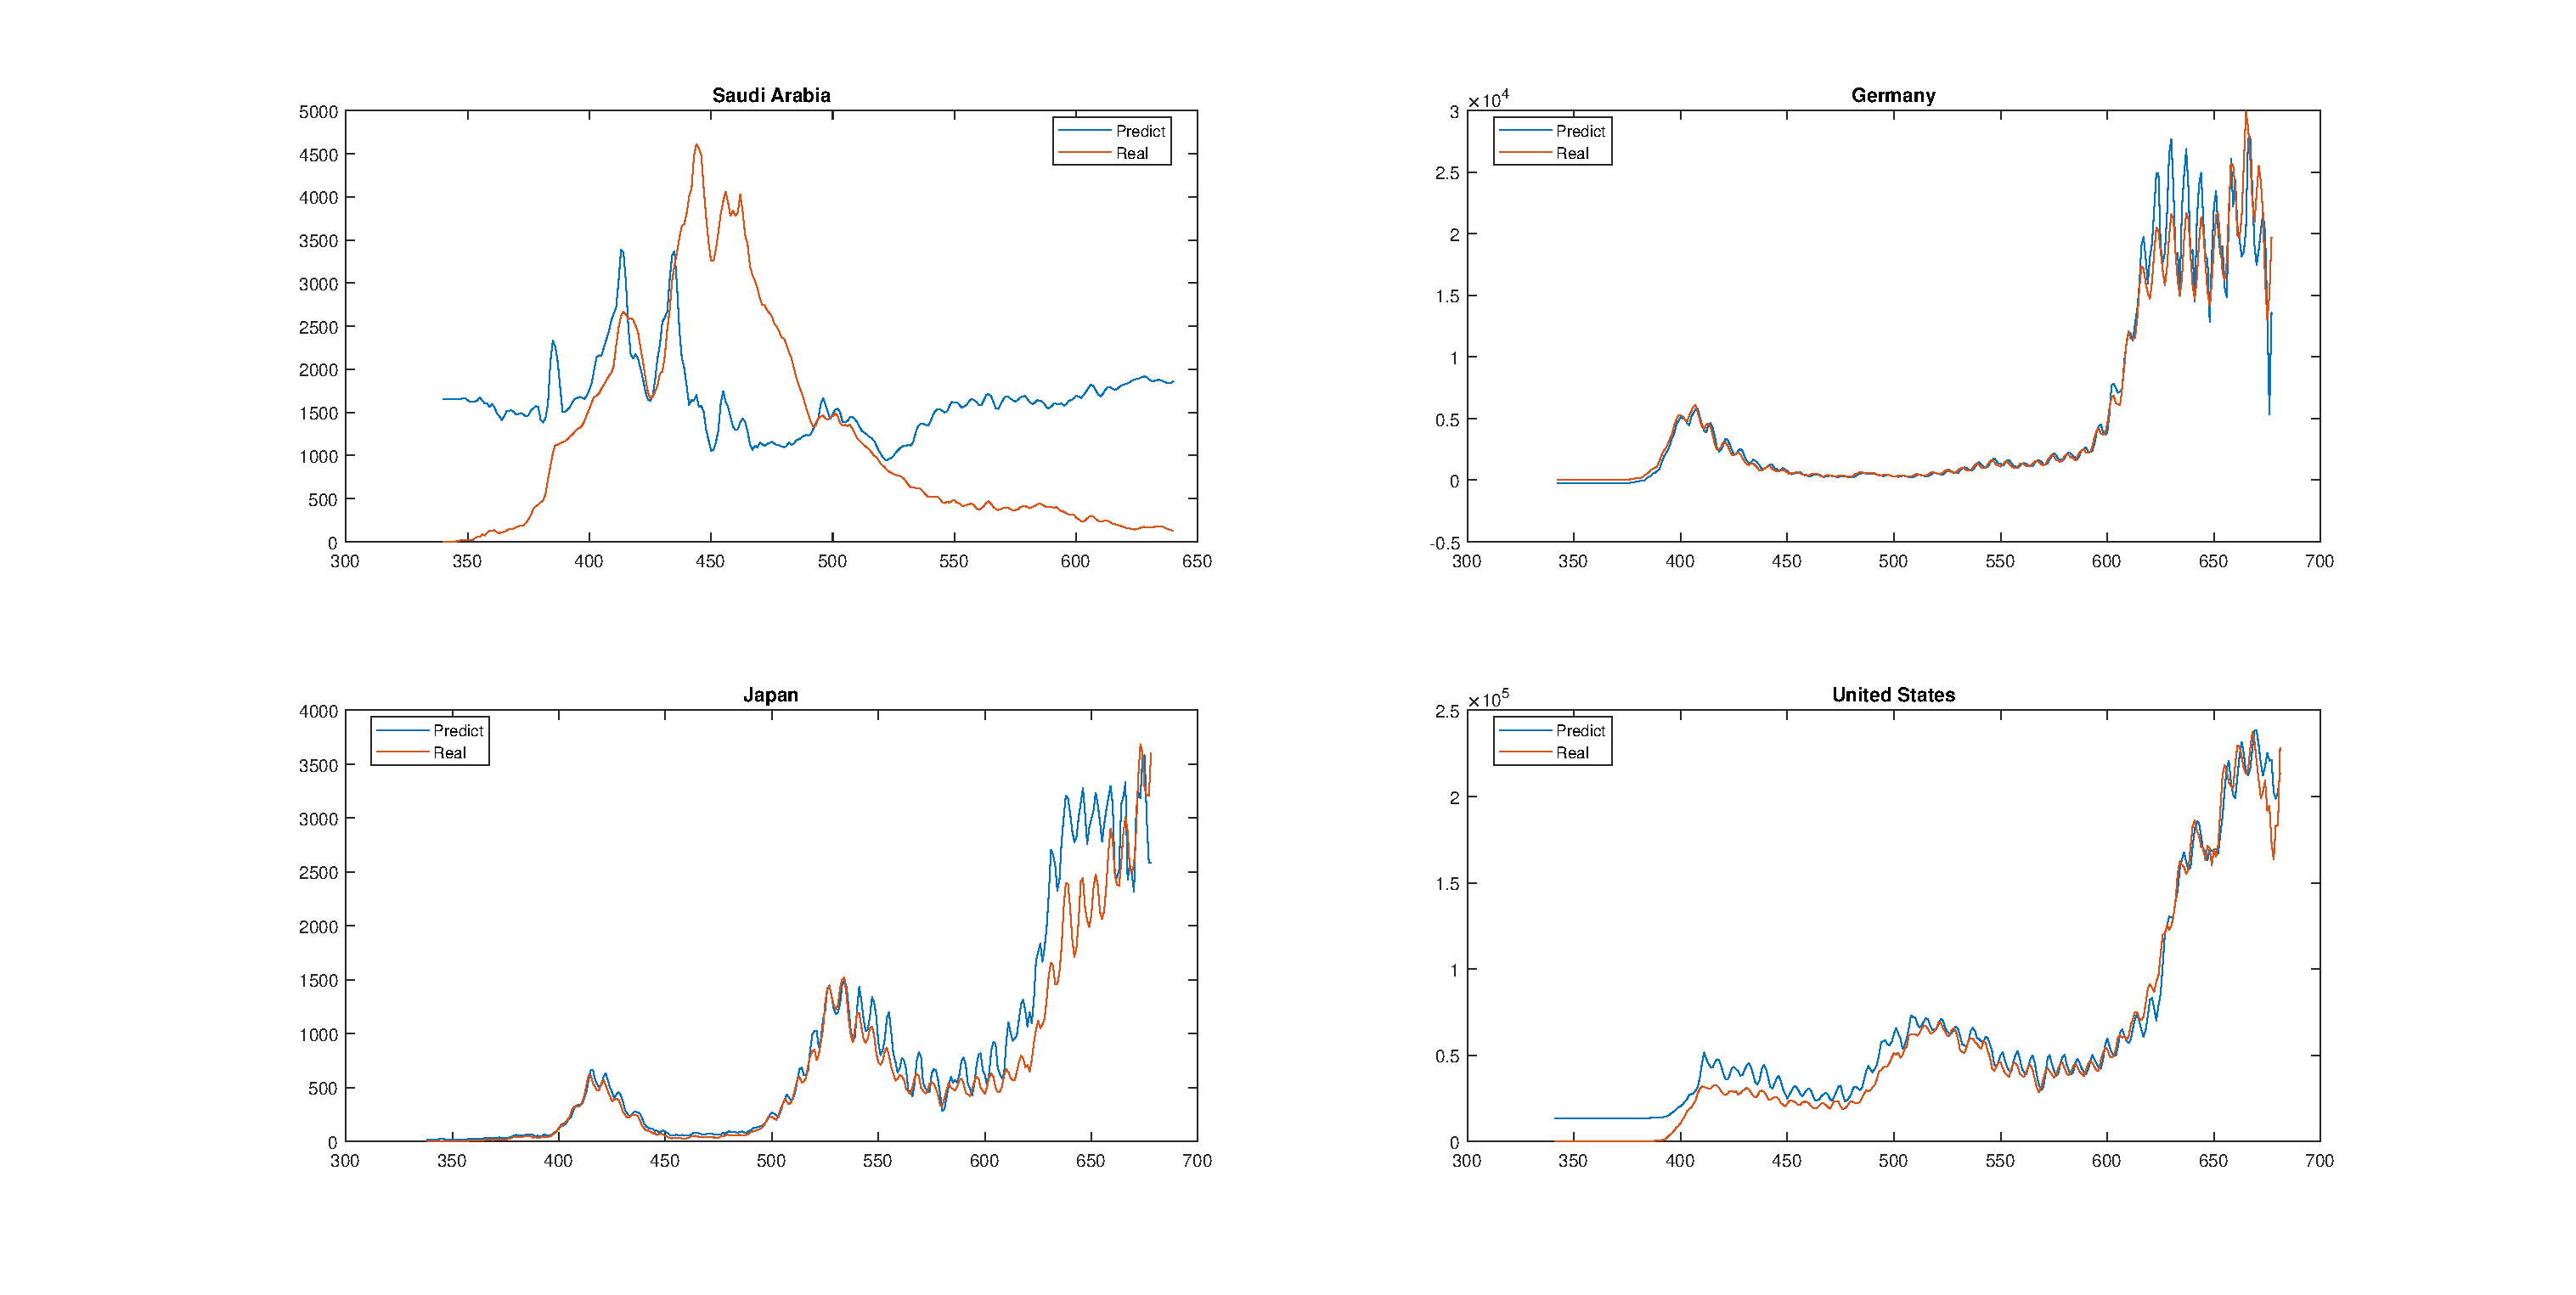
\includegraphics[height=12cm, width=14cm]{Pred2.eps}
	    }
	\end{figure}
	可以看到除了 Saudi Arabia 以外, 其余国家的拟合状况都是不错的; 注意到 Saudi Arabia 的疫情曲线也明显与其余几个国家有差别. 这一方面说明我们对国家的分类并不能完全说明其疫情的发展, 另外一方面说明我们的网络是 data-driven 的: 在并未见过这样疫情发展的情况下, 难以做出准确的预测. 如果我们在训练集中加上 China, Ethiopia, Zimbabwe 三个国家, 得到的结果将会有相当大的改善:
	\begin{figure}[htbp]
	    \centering
	    \subfigure{
	    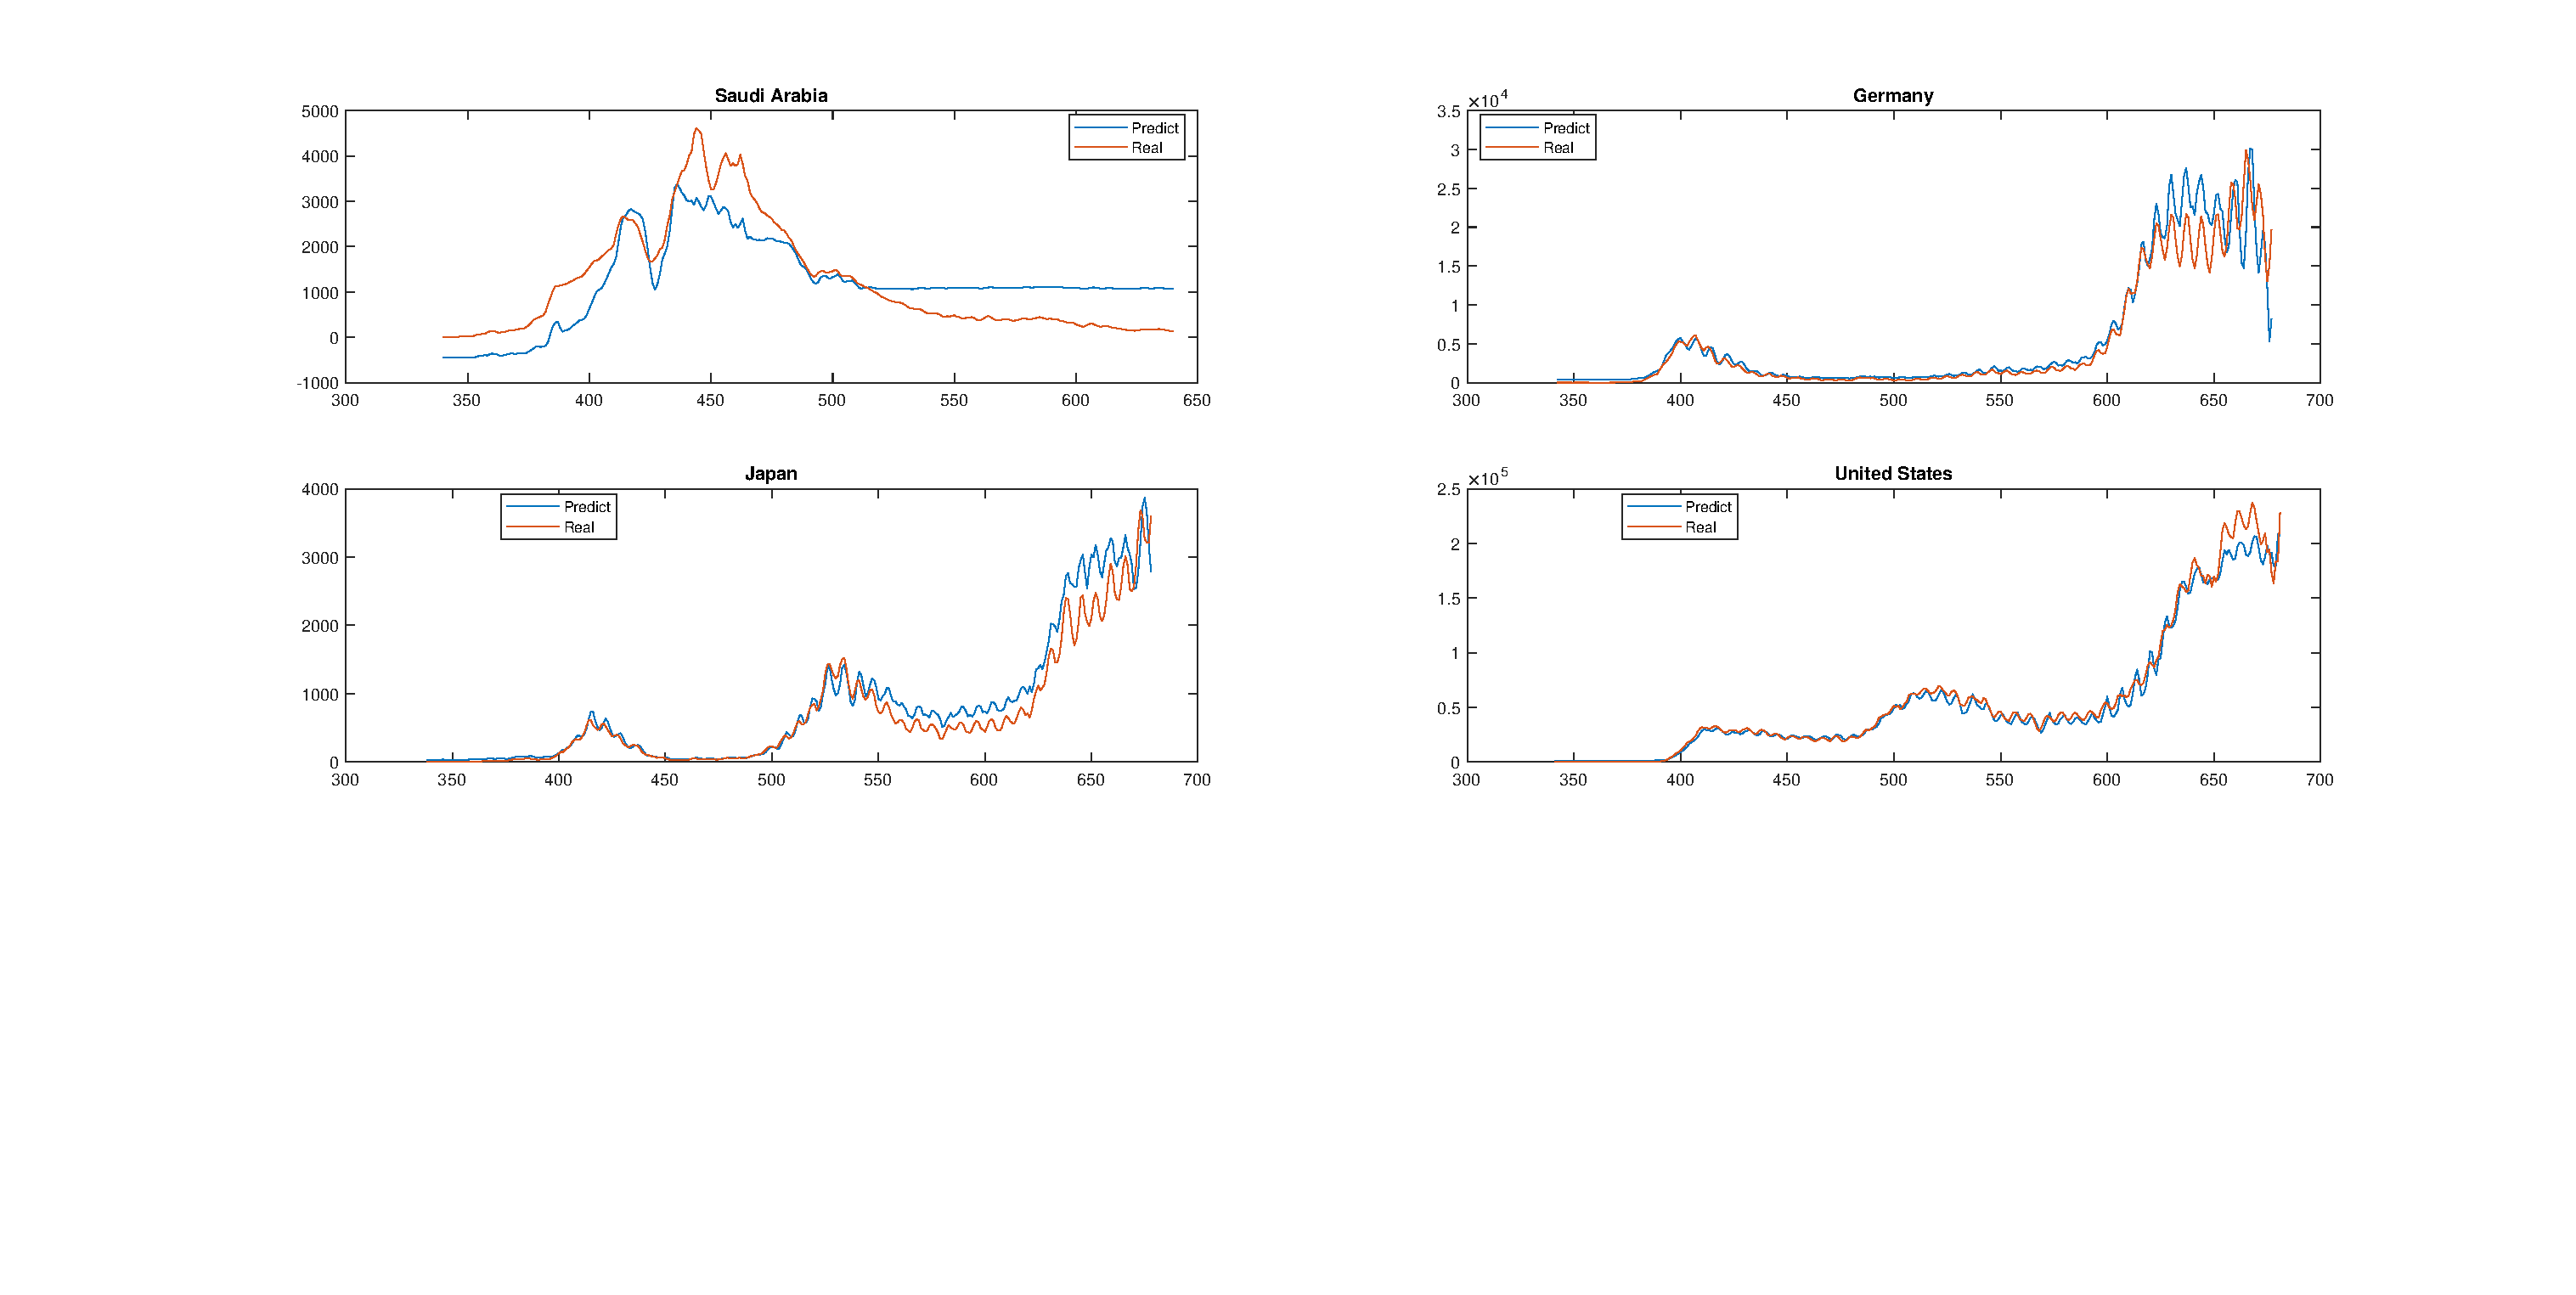
\includegraphics[height=12cm, width=14cm]{Pred3.eps}
	    }
	\end{figure}
	所以我们可以预见的是, 在数据越多的情况下, 我们能越好地预测疫情的发展状况.

	\subsubsection*{LSTM: 预测疫情发展状况}
    注意到在本次作业中, 并没有无症状携带者, 易感人群, 死亡病例等数据, 所以这里传统的 SEIR 或者 SEIRS 模型并不适用. 而新增病例是与时间有很强关系的数据, 我们选择 RNN 来进行预测是自然的. 这里我们选择 RNN 中的特殊种类——LSTM 进行预测. 同样地, 为方便起见, 也与 MATLAB 的风格相符, 我们直接列出网络结构:
	\begin{align*}
		&\text{sequenceInputLayer(8)} \rightarrow \\
    	&\text{fullyConnectedLayer(30)} \rightarrow \\
    	&\text{reluLayer} \rightarrow \\
    	&\text{lstmLayer(400)} \rightarrow \\
    	&\text{reluLayer} \rightarrow \\
    	&\text{fullyConnectedLayer(30)} \rightarrow \\
    	&\text{reluLayer} \rightarrow \\
    	&\text{fullyConnectedLayer(numResponses)} \rightarrow \\
    	&\text{regressionLayer}
	\end{align*}

    首先, 我们从不同的类别中挑出几个有代表性的国家, 这里我们的选取是 China, France, Ethiopia, Zimbabwe, Hungary, South Korea, Egypt, Australia, Canada, Iceland. 我们选取 Adam 优化器, 对上述数据训练 2000 个 epoches. 初始的学习率设置为 $0.001$, 并每 75 个 epoch 乘以 $0.95$. 同样地记新增病例数所称的向量为 $\mathcal{N}$, 我们使用
	\[
		\mathcal{N}_{\mathcal{S}} = \text{conv}(\mathcal{N},\mathcal{K}), \quad \mathcal{K} = \begin{bmatrix}
			\displaystyle\frac{1}{4}&\displaystyle\frac{1}{4}&\displaystyle\frac{1}{4}&\displaystyle\frac{1}{4}
	\end{bmatrix}
	\]
	我们将每日新增病例数与上面的核进行卷积, 考虑是两方面的: 一是为了方便网络的训练, 二是用四天的数据的平均来代替某一天的数据.
	在得到的数据中, 我们将前 $\frac{4}{5}$ 的病例数作为训练集, 将后 $\frac{1}{5}$ 的数据作为测试集. 可以看到效果是很好的.
	\begin{figure}[htbp]
	    \centering
	    \subfigure{
	    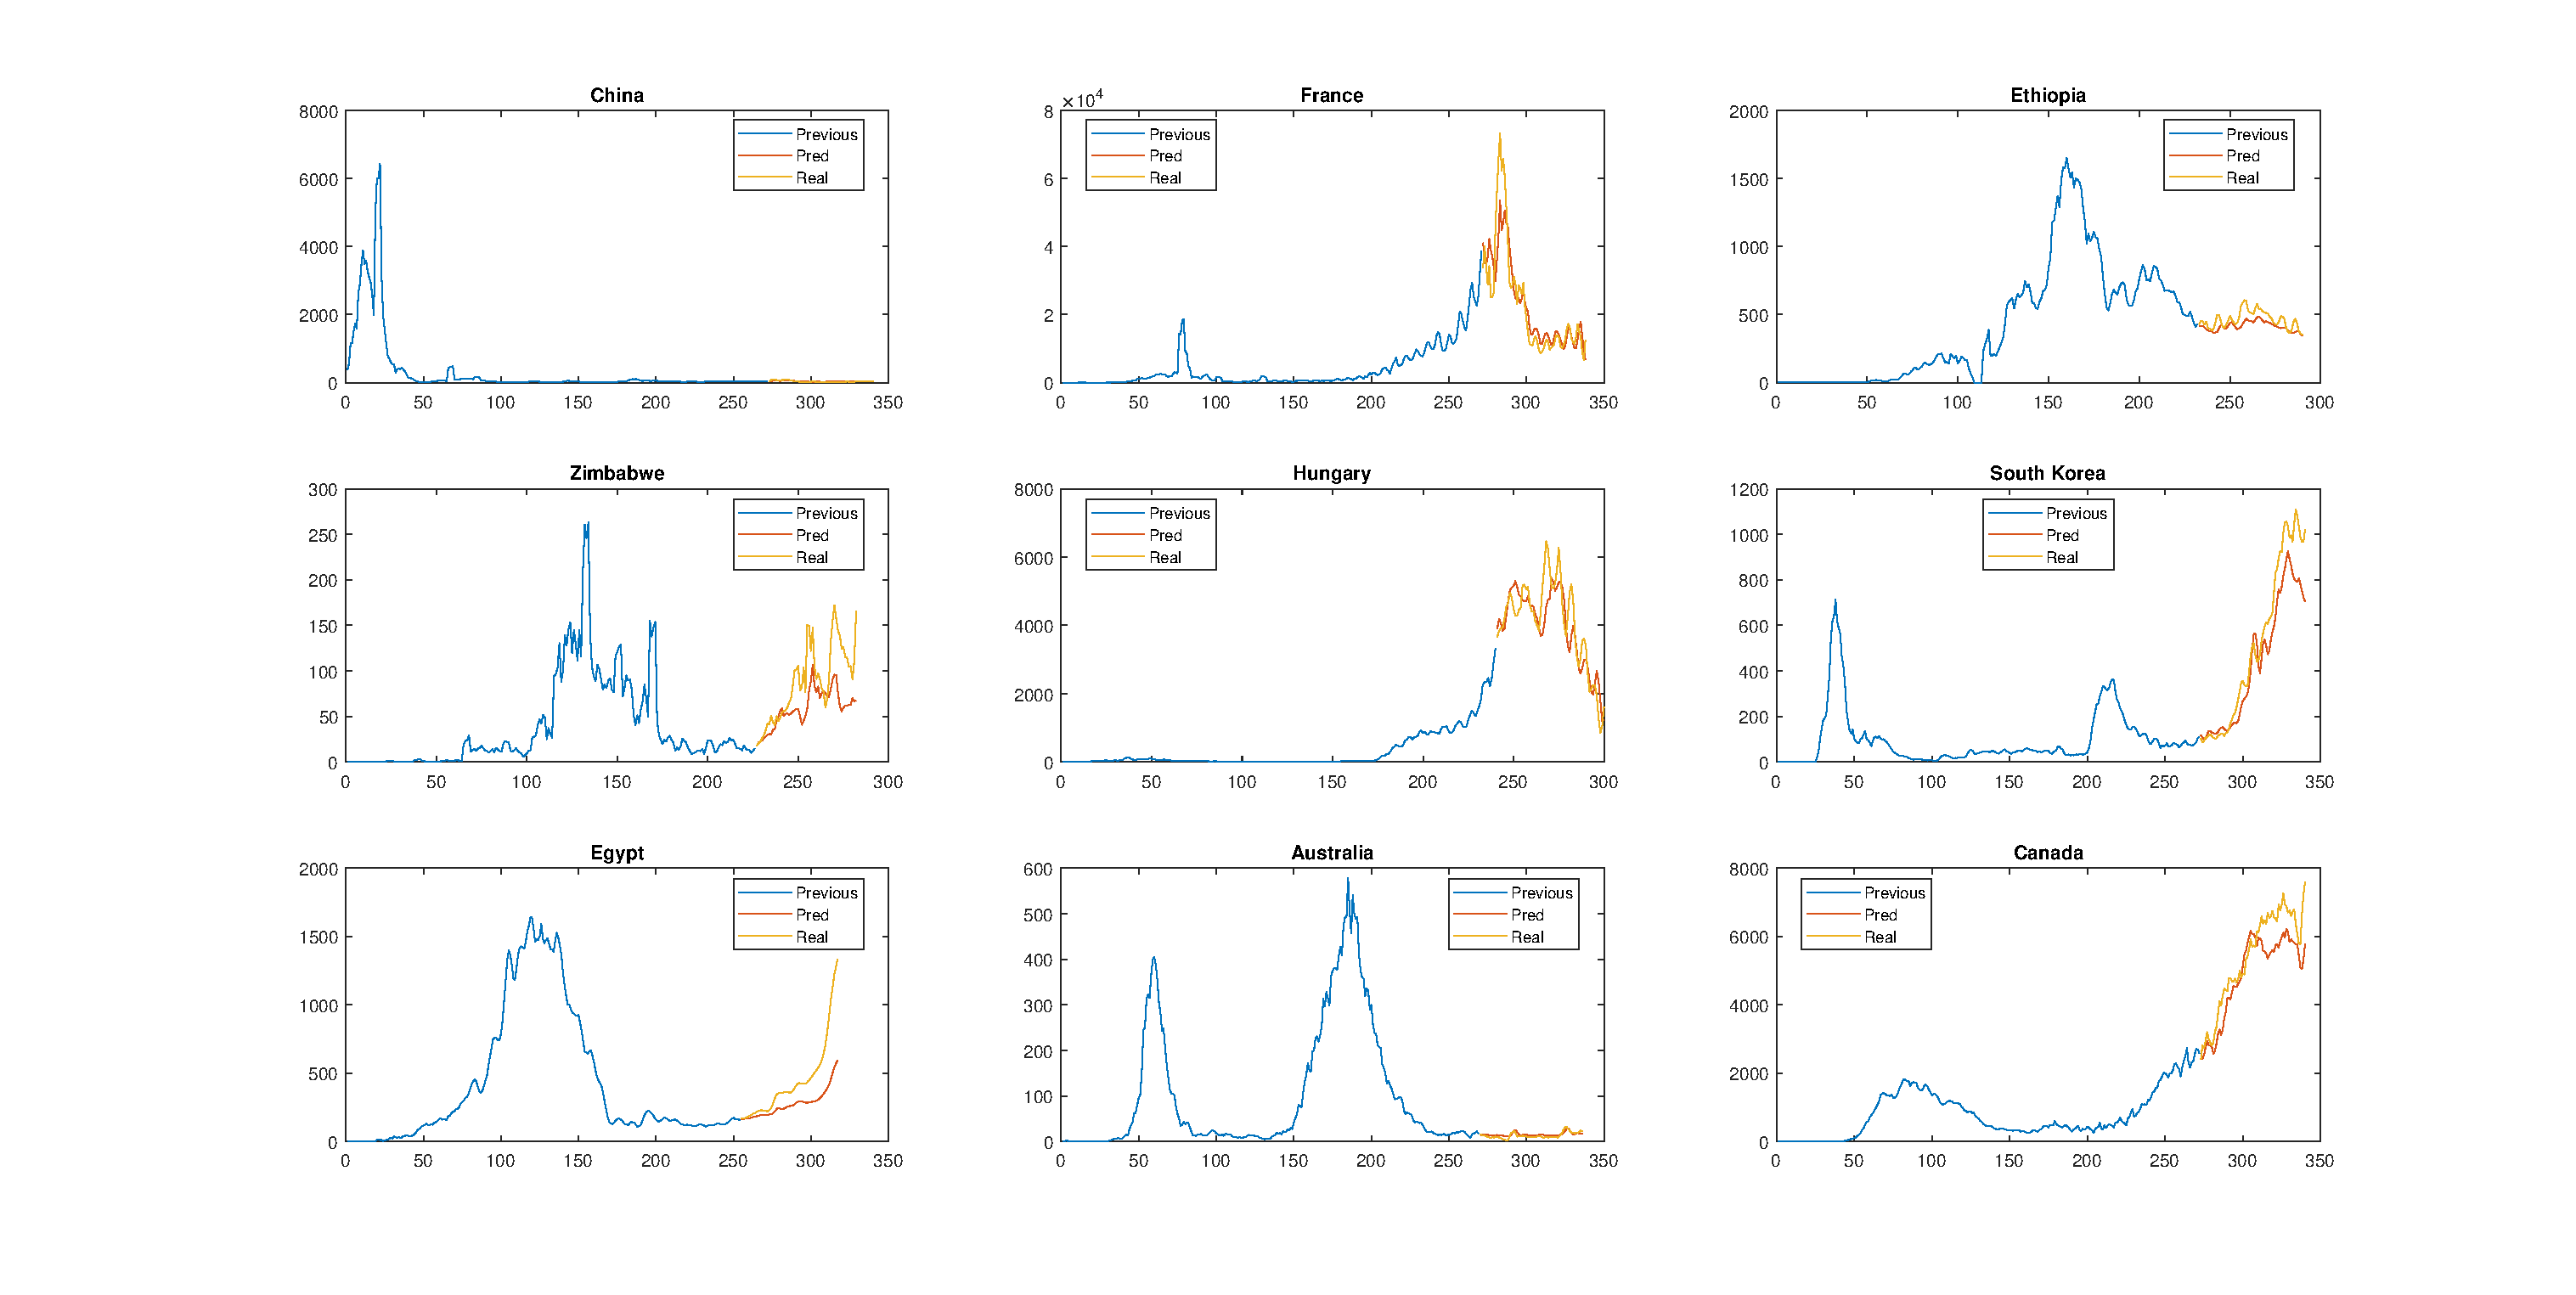
\includegraphics[height=12cm, width=14cm]{Pred.eps}
	    }
	\end{figure}
	这时我们相当于使用一个国家过去的疫情的发展信息来预测未来的发展. 我们想要看这个网络是否学到的是使用过去的信息, 抑或如果是没有见过的情况, 就难以处理? 注意到我们上面给出的例子, 我们使用 France, South Korea, Australia, Canada, Iceland 进行训练, 对 Saudi Arabia 进行测试:
	\begin{figure}[htbp]
	    \centering
	    \subfigure{
	    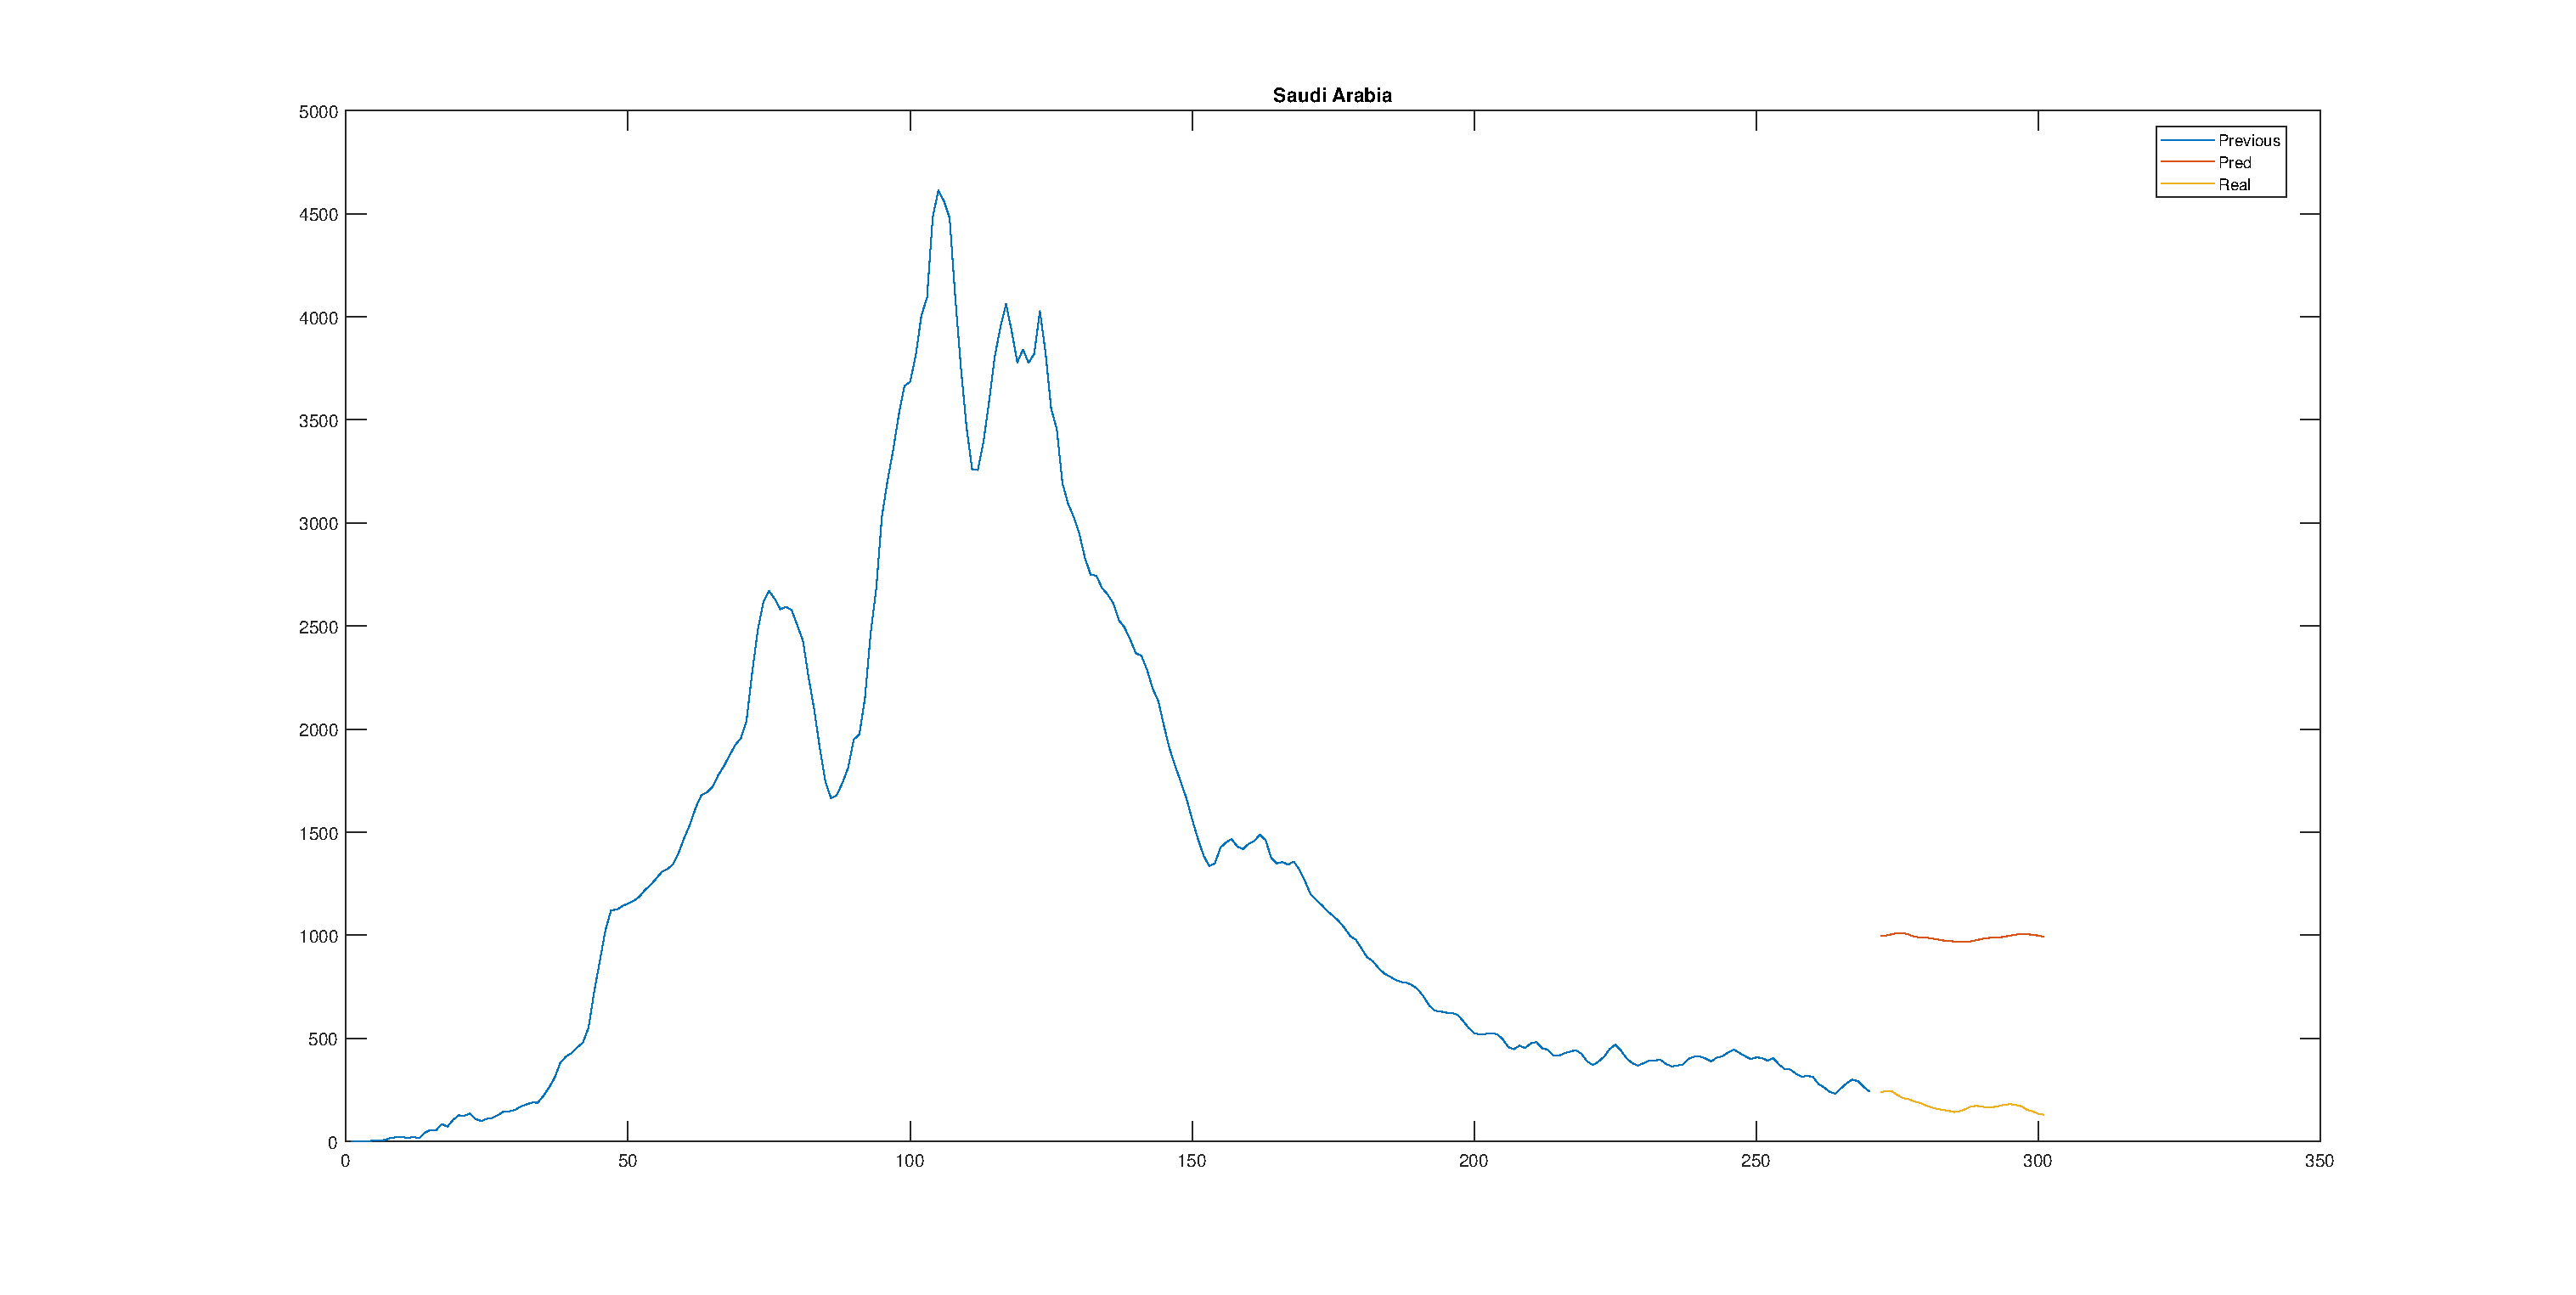
\includegraphics[height=12cm, width=14cm]{Pred4.eps}
	    }
	\end{figure}
	但是不幸的是仍然失败了. 这说明这样的 task 和我们所给出的数据对我们所构建的网络来说太难了. 想要达成我们所说的那种效果, 只能提升数据处理, 收集更多数据, 抑或是改变我们的网络的结构.
\end{document}
